\section{Problem Description}

In this project, we use a \ac{TDoA} approach to determine the location of the source of a wave on a 2-D plane, assuming direct line of sight from the source to the detector within the container (plane). The setup involves three sensor nodes placed at known locations \( S_i = (x_i, y_i) \), where \( i \in [1, 2, 3] \). The medium for wave propagation is water, with a measured wave speed \( v \). The source is located at an unknown position, \( P = (X, Y) \).

The detector array consists of three sensors placed on the boundaries of a 2-D plane, though can be placed anywhere. When the ToA is known, the distance from the source to each sensor can be calculated as
\begin{equation}
     d_{i} = v \cdot (t_i - t_0),
    \label{eqn:di}
\end{equation}
where \( t_0 \) is the time at which the signal is emitted, and \( t_i \) is the time at which the signal is received by sensor \( S_i \). From the distance a circle can be defined, centred at \( S_i \), and the intersection of these circles for three sensors gives the source location \cite{TDOA}, this is demonstrated in Figure \ref{fig:ToA}. However, in this scenario, the ToA from the detector to the sensor is not known, instead we rely on a different approach using the difference in time received between the three sensors as we have no knowledge of the emission time, the TDoA method.



\subsection{Time Difference of Arrival}

The TDoA method does not require knowledge of the emission time \( t_0 \). Instead, it uses the time differences \( \Delta t_{ij} \) between the arrival times at pairs of sensors, $i$ and $j$. These time differences are converted to distance differences \( \Delta d_{ij} \), which represents the path difference between $S_i$ and $S_j$ (Figure \ref{fig:path-diff}). Unlike the ToA method, which uses the resulting distance from Equation \ref{eqn:di} as the radius of three overlapping circles, the TDoA relies solely on $\Delta d_{ij}$ as the constant parameter. This can be used to form the basis of a hyperbolic equation as it represents a constant difference in distances from any point $(x,y)$ on the hyperbola to the two focal points $(x_i,y_i)$ and $(x_j,y_j)$, in this case the coordinates of the two associated detectors to $\Delta d_{ij}$. This hyperbola association forms part of our method to determining the location of the source as Figure \ref{fig:TDoA} shows how the solution to these hyperbolic equations is the location of the source. We will later discuss how this method introduces a degeneracy in the source position due to a second solution being present in certain cases. Due to this degeneracy a second method of localisation is used in conjunction with the prior method as a way of verifying calculations, this alternative method uses an iterative optimisation approach by applying the \lstinline[]{scipy.optimize.minimize} function.

\begin{figure}
    \centering
    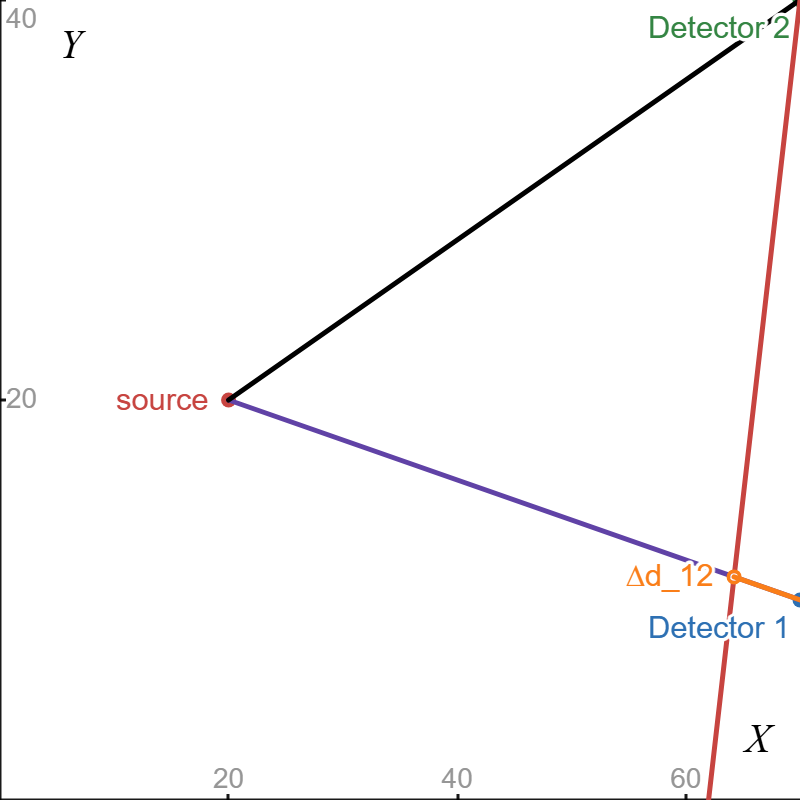
\includegraphics[width=0.5\linewidth]{images/desmos-graph.png}
    \caption{Visual representation of $\Delta d_{12}$ which is used in determining a source equation and a parameter of a hyperbolic equation.}
    \label{fig:path-diff}
\end{figure}

\begin{figure}[h!]
    \centering
    \begin{subfigure}[b]{.5\textwidth}
      \centering
      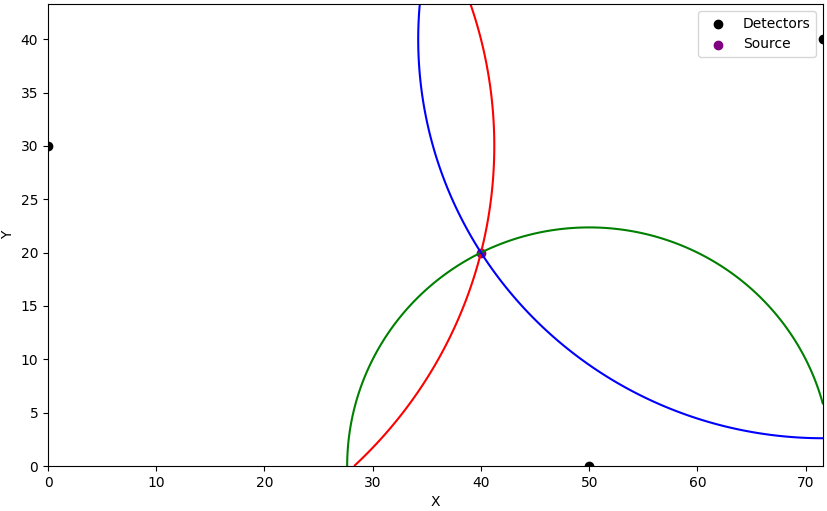
\includegraphics[width=\textwidth]{images/Figure_11.png}
      \caption{}
      \label{fig:ToA}
    \end{subfigure}%
    \begin{subfigure}[b]{.485\textwidth}
      \centering
      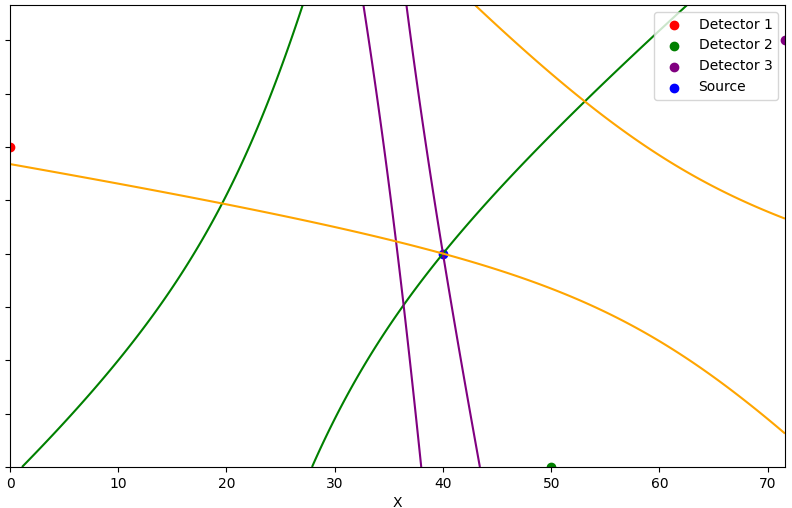
\includegraphics[width=\textwidth]{images/Figure_22.png}
      \caption{}
      \label{fig:TDoA}
    \end{subfigure}
    \caption{Visualisation of ToA and TDoA measurements. (\textbf{a}) ToA measurements when the time of emission is known at the source. (\textbf{b}) TDoA measurements crossing at the source of emission.}
    \label{fig:TDoA-ToA}
\end{figure}
\newpage

For three sensors, the distance differences are given by:

\begin{equation}
\Delta d_{12} = v \cdot (t_2 - t_1)
\label{eqn:dd_12}
\end{equation}

\begin{equation}
\Delta d_{13} = v \cdot (t_3 - t_1)
\label{eqn:2.2}
\end{equation}

As $\Delta d_{ij}$ is a path difference, by definition it also relates to the difference in distances between the source and detector 1 and 2, $d_1, d_2$.

\begin{equation}
    \Delta d_{ij} = d_j - d_i
    \label{eqn:d_ij}
\end{equation}

where $d_i$ can be defined as

\begin{equation}
    d_i = \sqrt{(x-x_i)^2+(y-y_i)^2}
    \label{eqn:d_i}
\end{equation}

substituting Equation \ref{eqn:d_i} into Equation \ref{eqn:d_ij} yields a hyperbolic equation where the solution is the source location \cite{s19112554}

\begin{equation}
\sqrt{(x - x_2)^2 + (y - y_2)^2} - \sqrt{(x - x_1)^2 + (y - y_1)^2} = \Delta d_{12}
\label{eqn:dd12}
\end{equation}

\begin{equation}
\sqrt{(x - x_3)^2 + (y - y_3)^2} - \sqrt{(x - x_1)^2 + (y - y_1)^2} = \Delta d_{13}.
\label{eqn:dd13}
\end{equation}

\begin{equation}
    \sqrt{(x - x_3)^2 + (y - y_3)^2} - \sqrt{(x - x_2)^2 + (y - y_2)^2} = \Delta d_{13}.
\label{eqn:dd23}
\end{equation}

In order to determine $P$ we must solve these hyperbolic equations, i.e. where they intersect. There are many ways to solve these equations, such as the approximate maximum likelihood method \cite{1583909} which can calculate solutions to a linear maximum likelihood equation. In this project we use something similar, an iterative optimisation approach to find the source position, utilising the \lstinline{scipy} library.

\subsection{Source Location Problem}
\label{subsec:2.1.2}

To localise the source, we formulate an objective function \( f(x, y) \) that quantifies the discrepancy between the calculated and observed distance differences.

\begin{equation}
f(x, y) = (d_2 - d_1 - \Delta d_{12})^2 + (d_3 - d_1 - \Delta d_{13})^2
\label{eqn:SF}
\end{equation}

The goal is to find the source position \( (x, y) \) that minimises \( f(x, y) \). This ensures that the calculated distance differences match the observed distance differences as closely as possible. In layman's terms this is determined by iteratively inputting different values of $(x,y)$ and checking the numerical result of Equation \ref{eqn:SF} until it approaches zero, whereby the source has been localised. This comes as a result of Equation \ref{eqn:dd12} approaching Equation \ref{eqn:dd_12}, ditto for sensors 1 and 3, as the calculated distance difference approaches the measured difference.

The minimisation of \( f(x, y) \) is performed using the \lstinline{scipy.optimize.minimize} function which uses an iterative, gradient-based optimisation algorithm, such as BFGS \cite{BFGSscipy} \cite{enwiki:1273231919}. The process begins with an initial guess for the source position, defined to be:

\begin{equation}
(x_0, y_0) = \left( \frac{x_1 + x_2 + x_3}{3}, \frac{y_1 + y_2 + y_3}{3} \right)
\end{equation}

The algorithm evaluates the objective function and its gradient at the guess and updates the guess in the direction that reduces \( f(x, y) \). This process repeats until convergence is achieved, meaning the change in \( f(x, y) \) approaches zero. The result is the estimated source position \( (X, Y) \) that minimises the objective function, resulting from the source function producing a singular point where the objective function is as close to zero as possible.

\subsubsection{Physical Interpretation of the Source Function}
The objective function \( f(x, y) \) represents the total error in the distance differences for a given source position. When \( f(x, y) = 0 \), the calculated distance differences exactly match the observed distance differences, indicating that the source position is perfectly consistent with the data. In practice, \( f(x, y) \) is rarely zero due to measurement uncertainties and noise, minimising it provides the best estimate of the source location.

The source function can be visualised (Figure \ref{fig:source-func}) as an array of contour lines to show how the function behaves over space. Each line represents regions where the function has the same value, where the minimum of the function corresponds to the point where the contour lines' value approach zero. The spread in the lines gives an indication of the uncertainty in the source propagation.

\begin{figure}
    \centering
    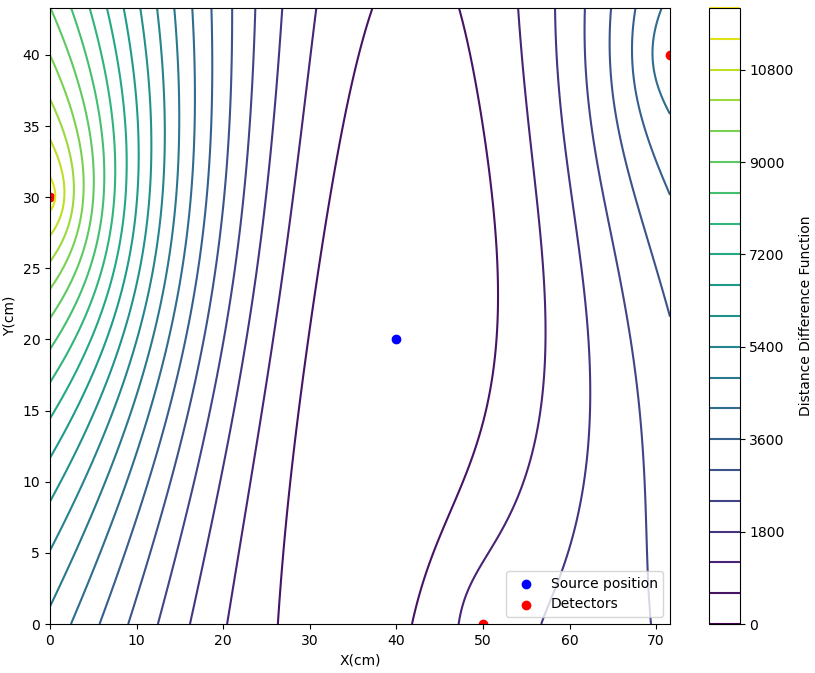
\includegraphics[width=0.75\linewidth]{images/source-func.png}
    \caption{Visualisation of the source localisation process. The contour lines represent the distance difference function, with the minimum corresponding to the source position \cite{boxer_2025_15041819}.}
    \label{fig:source-func}
\end{figure}

The use of squared differences in the objective function ensures that the function is smooth and differentiable, making it suitable for gradient-based optimisation methods. Additionally, squaring the differences penalises larger discrepancies more heavily, encouraging the optimiser to find a solution where the calculated and observed differences are as close as possible.

\subsection{Hyperbola Association}
\label{sec:hyp-ass}

In Figure \ref{fig:TDoA} the hyperbola are plotted using Equations \ref{eqn:dd12}-\ref{eqn:dd12}, where the solution to the three hyperbola equations are the possible locations of the source. In most cases there is only one solution to the equation within the plane, usually occurring when the source is located around the centre of the plane. In some cases two solutions arise within the plane, as is the case in Figure \ref{fig:2-loc}, this degeneracy is a result of the square root factor of the equation producing two branches. To eliminate this degeneracy an extra detector can be used, in Figure \ref{fig:4-det} a fourth detector demonstrates how the source location can be determined from the intersection of all four hyperbolas. Compared to Figure \ref{fig:2-loc} where the three hyperbolic equations intersect at two points within the plane, Figure \ref{fig:4-det} introduces an extra hyperbolic equation (shown in blue) resulting from the TDoA between detector 4 and 1.

\begin{figure}[h!]
    \centering
    \begin{subfigure}[b]{.5\textwidth}
      \centering
      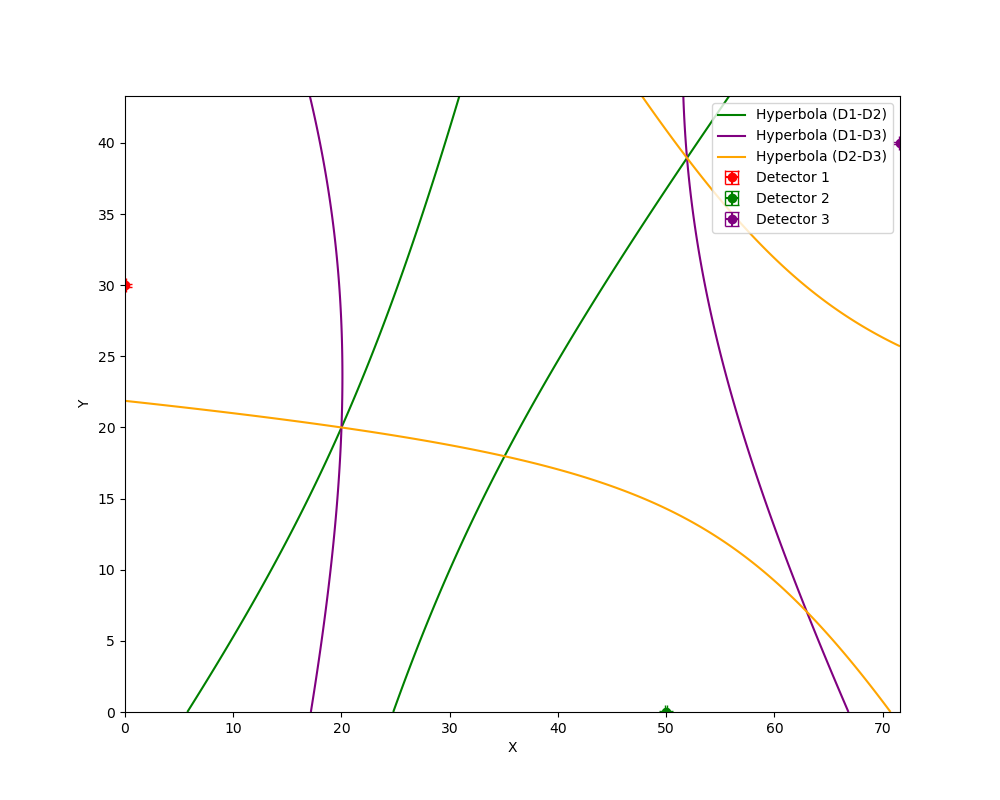
\includegraphics[width=\textwidth]{images/2-loc.png}
      \caption{}
      \label{fig:2-loc}
    \end{subfigure}%
    \begin{subfigure}[b]{.5\textwidth}
      \centering
      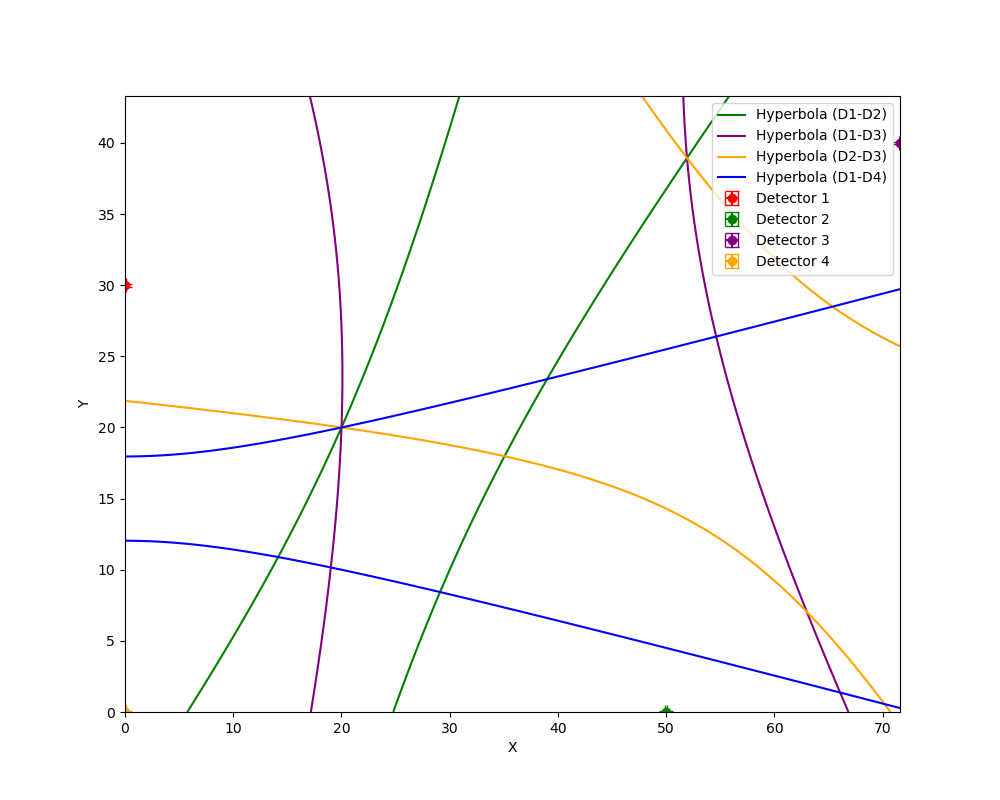
\includegraphics[width=\textwidth]{images/4-det.png}
      \caption{}
      \label{fig:4-det}
    \end{subfigure}
    \caption{Degernacy elimination by adding fourth detector. (\textbf{a}) Cases where there are two solutions of the hyperbolic equations within the plane, despite only one solution containing the source. (\textbf{b}) Degeneracy elimination using a fourth detector placed at $(0,0)$, where all four intersect represents the location of the source.}
    \label{fig:TDoA-ToA}
\end{figure}
\newpage


\subsection{Uncertainty Analysis} 

In addition to determining the source position, it is crucial to quantify the uncertainty in the calculated location due to errors in the measured time differences and sensor positions. This uncertainty arises from various sources, including measurement noise, sensor placement errors, and uncertainties in the wave speed \( v \).

For a given pair of detectors, the time difference \(\Delta t_{ij}\) corresponds to a distance difference \(\Delta d_{ij} = v \cdot \Delta t_{ij}\), where \(v\) is the wave propagation speed. We assume Gaussian uncertainties since many measurement errors follow a normal distribution, especially in this case where they result from the combination of many small, independent sources of error \cite{enwiki:1251161789}, such as in timing uncertainties in measuring the arrival time. It is beneficial to assume Gaussian uncertainties due to their additivity too where the sum of independent Gaussian random variables is also Gaussian.

The uncertainty in \(\Delta d_{ij}\) arises from the uncertainties in the arrival times and the wave speed. For example, the uncertainty in \(\Delta d_{12}\) is calculated as:

\begin{equation}
\delta (\Delta d_{12}) = \sqrt{(v \cdot \delta t_1)^2 + (v \cdot \delta t_2)^2 + (\Delta t_{12} \cdot \delta v)^2},
\label{eqn:dd12-unc}
\end{equation}

where \(\delta t_1\), \(\delta t_2\), and \(\delta v\) are the uncertainties in \(t_1\), \(t_2\), and \(v\), respectively. This uncertainty is propagated to the hyperbola equation \ref{eqn:dd12}. The uncertainty in the hyperbola is visualised by plotting contours corresponding to \(\Delta d_{12} \pm \delta (\Delta d_{12})\).

\newpage


